The tool selection page necessitates the user to choose the underlying tool for
the decomposition process. Currently, the only implemented tool available for
selection is the one developed by Miguel Brito
\citeSLR{brito2021identification}.

\Cref{fig:tool_selection,fig:project_upload,fig:awaiting_decomposition}
visually depict the step-by-step procedure involved in selecting a tool,
uploading a file, and waiting for the decomposition to be performed. These
illustrations provide a clear representation of the user interface and the
corresponding actions taken by the user during the tool selection process.
\Cref{fig:tool_selection} showcases the tool selection interface, where the user
can choose the desired tool. \Cref{fig:project_upload} exhibits the file upload
functionality, allowing the user to upload a file that contains the project to
be decomposed. Finally, \Cref{fig:awaiting_decomposition} illustrates the
waiting process as the system performs the decomposition, providing the user
with a progress indicator or other relevant information.

\begin{figure*}[!htb]
  \caption{Tool Selection}
  \label{fig:tool_selection}
  \centering
  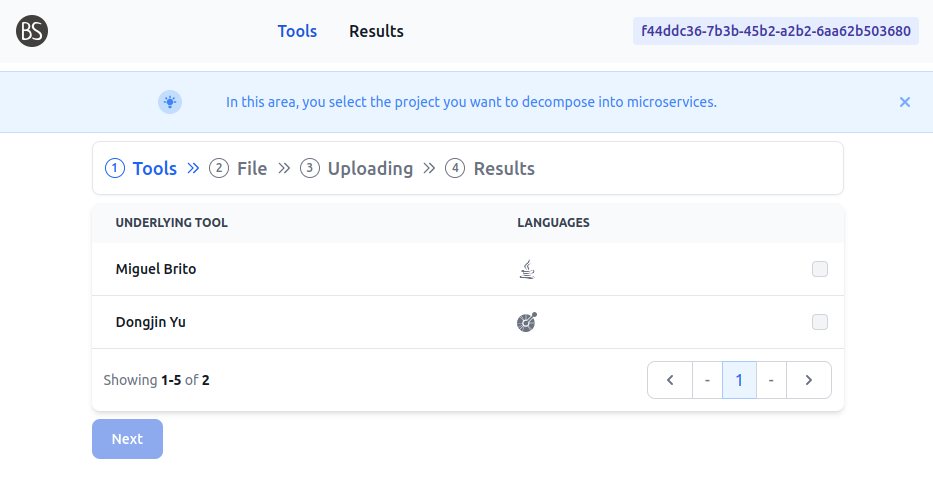
\includegraphics[width=\textwidth]{tools_selection}
\end{figure*}
\begin{figure*}[!htb]
  \caption{Project Upload}
  \label{fig:project_upload}
  \centering
  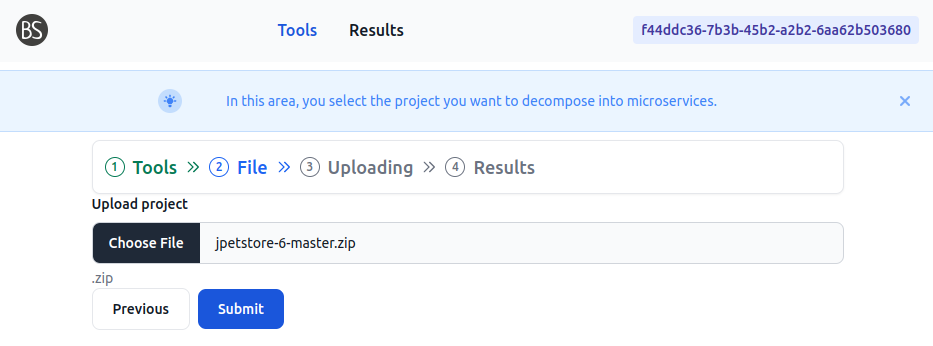
\includegraphics[width=\textwidth]{tools_project_upload}
\end{figure*}
\begin{figure*}[!htb]
  \caption{Awaiting Decomposition}
  \label{fig:awaiting_decomposition}
  \centering
  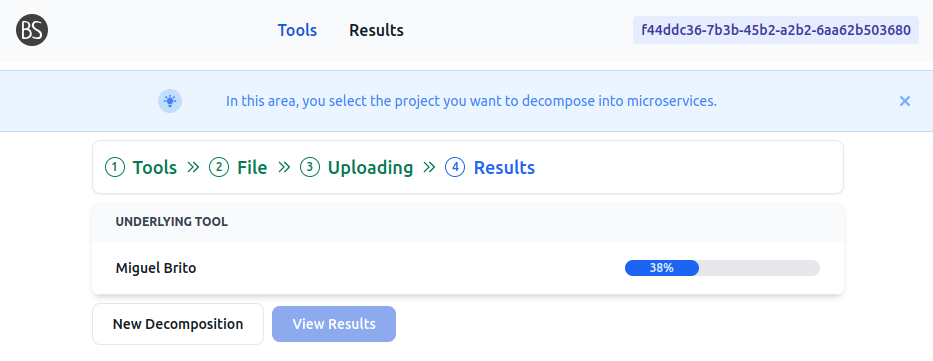
\includegraphics[width=\textwidth]{tools_awaiting_decomposition}
\end{figure*}
